\section{Projekt Infrastruktury Sieciowej}

\subsection{Schemat logiczny sieci}
        
    \begin{figure}[!htb]
        \centering
        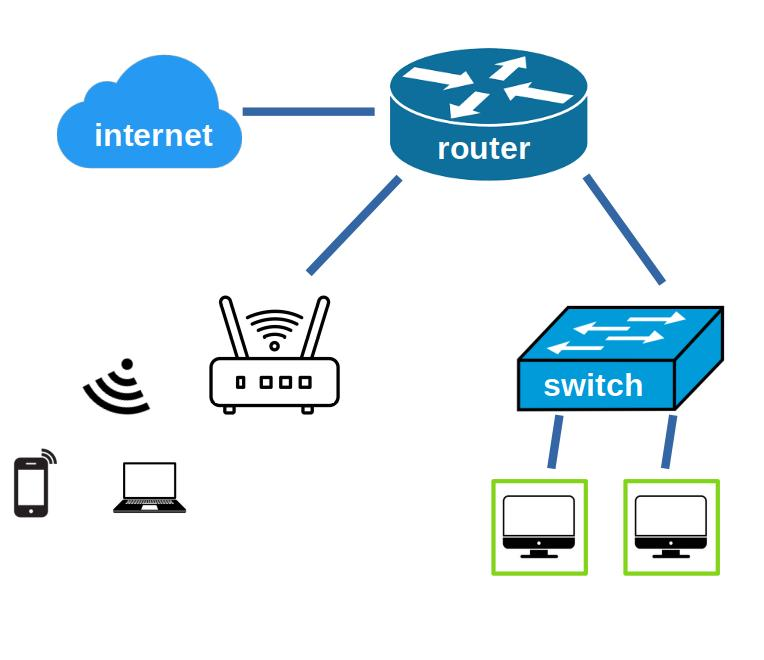
\includegraphics[width=0.6\textwidth]{schematy/logiczny}
        \caption{Schemat logiczny sieci}
    \end{figure}

\subsection{Projekt sieci - Cisco Packet Tracer}
    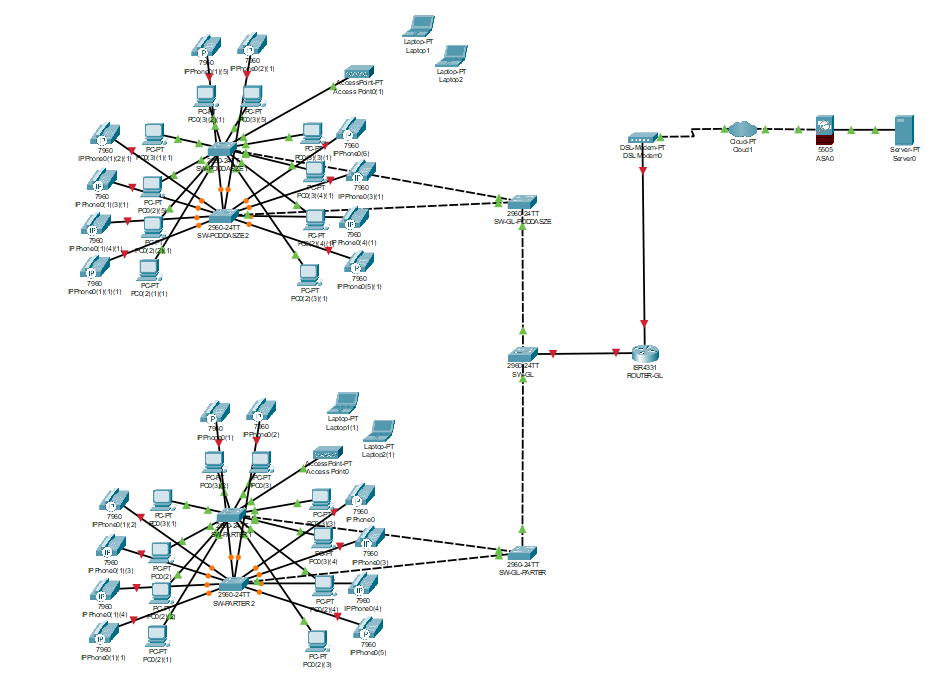
\includegraphics[width=1.0\textwidth]{schematy/cisco.png}

\pagebreak

\subsection{Topologia Sieci}

    W projekcie infrastruktury sieciowej proponujemy zastosowanie topologii sieci opartej na modelu gwiazdy. Każde stanowisko komputerowe, w tym stacje robocze i stacje administracyjne, będzie podłączone bezpośrednio do centralnego przełącznika (switcha). To rozwiązanie zapewnia prostą skalowalność i łatwe zarządzanie siecią.

        
    \begin{figure}[!htb]
        \centering
        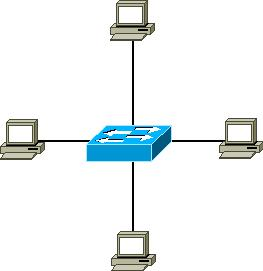
\includegraphics[width=0.3\textwidth]{gwiazda}
        \caption{Topologia Gwiazdy}
    \end{figure}


\subsection{Kable i Media Transmisyjne}

    Do połączenia urządzeń w sieci użyjemy kabli UTP kategorii 6e o odpowiedniej długości. Ponadto, w niektórych przypadkach zastosujemy kable światłowodowe, zwłaszcza tam, gdzie potrzebna jest duża przepustowość, na przykład między centralnym serwerem zasobów a głównym switchem.

\subsection{Urządzenia Sieciowe}
    W naszym projekcie użyjemy następujących urządzeń sieciowych:
    \begin{itemize}
        \item - Centralny przełącznik (switch) do obsługi wszystkich stanowisk.
        \item Router zapewniający dostęp do internetu oraz segregację sieci wewnętrznej i sieci gości.
        \item Access Pointy Wi-Fi dla zapewnienia dostępu do sieci bezprzewodowej.
        \item Firewall do zabezpieczenia sieci przed nieautoryzowanym dostępem.
    \end{itemize}



\subsection{Zapotrzebowanie na Przepustowość}

    Na podstawie analizy potrzeb firmy określiliśmy zapotrzebowanie na przepustowość sieci. Oceniliśmy, że przepustowość 1 GbE (Gigabit Ethernet) będzie wystarczająca dla stanowisk komputerowych, biorąc pod uwagę typowe obciążenia sieciowe w firmie. 
    Naszym operatorem zostanie firma ORANGE\\ \\
    \url{https://oferty.orange.pl/swiatlowod/koszalin}
    
\includegraphics[width=0.1\textwidth]{orange} \\
